\chapter{Approximation}
\lecture{13}{12 Dec. 14:20}{}

\section{Approximation Algorithm}

對於 NP-Hard 問題,我們通常無法在多項式時間內找到最佳解,因此我們可能可以將問題簡單化,或是使用啟發式演算法 (heuristic algorithm) 來找到近似解 (approximate solution),犧牲掉一些的最佳性,來換取更快的運算時間。但 approximate algorithm 並不是 heuristic algorithm,而針對 approximate algorithm,我們有一些要求:
\begin{itemize}
    \item 針對最佳化問題(optimization problems):目標是尋找最佳解(optimal solution),而非回答「是」或「否」的 decision problems
    \item 必須是 polynomial-time algorithm
    \item 必須保證解的品質(quality of solution):這是與 heuristic algorithm 最大的不同點
\end{itemize}

衡量 approximate algorithm 的標準是 approximation ratio,定義如下:
\begin{definition}[Approximation Ratio]
    For a minimization problem, let $C$ be the cost of the solution returned by an approximate algorithm, and $C^*$ be the cost of an optimal solution. An algorithm is said to have an approximation ratio of $\rho(n)$ if for all instances of size $n$, it holds that
    \[
        \frac{C}{C^*} \leq \rho(n)
    \]
    For a maximization problem, the approximation ratio is defined as
    \[
        \frac{C^*}{C} \leq \rho(n)
    \]
\end{definition}

\begin{remark}
    通常我們希望 $\rho(n)$ 越接近 1 越好,若 $\rho = 1$ 則這是最佳演算法
\end{remark}

\begin{note}
    也存在 additive guarantee 的定義方式 \[
        |C - C^*| \leq k
    \]
    但很難達到
\end{note}

\newpage

\subsection{Vertex Cover Problem}

\begin{exercise}[Vertex Cover (Optimization Version)]
    Given
    \begin{itemize}
        \item \textbf{Input}: A graph $G = (V, E)$.
        \item \textbf{Output}: A vertex cover $S$ of $G$ with minimum $|S|$.
    \end{itemize}
\end{exercise}

\begin{algorithm}
    \DontPrintSemicolon % 隱藏每行句尾的分號 ;
    
    % 定義輸入輸出
    \KwIn{A graph $G = (V, E)$}
    \KwOut{A vertex cover $C$ of $G$}

    $C \leftarrow \emptyset$\;
    $E' \leftarrow E(G)$\;
    \While{$E' \neq \emptyset$}{
        $(u, v) \leftarrow \text{an arbitrary edge from } E'$\;
        $C \leftarrow C \cup \{u, v\}$\;
        $E' \leftarrow E' \setminus \{ \text{edges incident to } u \text{ or } v \}$\;
    }
    \Return $C$\;

    \caption{Approximation Algorithm for Vertex Cover}
\end{algorithm}

對於每個邊 $(u, v)$,我們都將 $u$ 和 $v$ 加入 vertex cover $C$ 中,但對於 optimal cover $C^*$ 來說,只需要 $u$ 或 $v$ 即可,因此我們可以得到 \[
    |C| \leq 2 \cdot |C^*|
\]
並且他的運行時間是 $O(|V| + |E|)$,所以這是一個 \textbf{2-approximation algorithm}

\begin{note}
    兩倍其實沒有高估,對於 worst-case 來說
    \begin{figure}[H]
        \centering
        \begin{tikzpicture}[auto]
            \node [state] (a1) at (0, 0) {$p_1$};
            \node [state] (a2) at (3, 0) {$p_2$};
            \node [state] (b1) at (0, -1) {$q_1$};
            \node [state] (b2) at (3, -1) {$q_2$};
            \node [state] (c1) at (0, -2) {$r_1$};
            \node [state] (c2) at (3, -2) {$r_2$};

            \draw (a1) -- (a2);
            \draw (b1) -- (b2);
            \draw (c1) -- (c2);
        \end{tikzpicture}
        \caption{Worst-case for Approximation Algorithm for Vertex Cover}
    \end{figure}
    optimal cover 只需要選擇 $\{p_1, q_1, r_1\}$,但 approximation algorithm 可能會選擇 $\{p_1, p_2, q_1, q_2, r_1, r_2\}$
\end{note}

\begin{remark}[Upper Bound and Lower Bound]
    目前已知的 vertex cover approximation algorithm 的最佳 approximation ratio 為 $2 - \epsilon$ for $\epsilon = 1$ 例如 Karakostas 的 \[
        2 - \Theta\left(\frac{1}{\sqrt{\log n}}\right)
    \]
    在 $P \neq NP$ 的前提下,已知的 lower bound 為 P-time approximation ratio 最高的是 \[
        \sqrt{2} \approx 1.414
    \]
\end{remark}

\vspace{1em}

有時候 Greedy Algorithm 並不一定是好的 approximate algorithm,如果我們採用 Greedy Algorithm 來解決 vertex cover 問題,會發現他並不是一個好的 approximate algorithm,因為在 worst-case 下,他的 approximation ratio 可能會高達 $\Theta(\log n)$,並且是 tight 的分析,如果我們採用的 Greedy 策略是 \begin{quotation}
    Repeatedly select the vertex $v$ with \[
        \max_{v \in V} \deg(v)
    \]
\end{quotation}

The worst-case can be get by an Bipartite Graph ($G = (L \cup R, E)$) as follows:

Build a bipartite graph $G = (L \cup R, E)$ where \[
    L: |L| = k
\]
and 
\[
    R: R = \bigcup_{i=1}^{k} R_i, \text{ where } |R_i| = \left\lfloor \frac{k}{i} \right\rfloor
\]

在這個 case 底下,optimal cover 只需要選擇 $L$,但 Greedy Algorithm 會先選擇 $R_1$,接著是 $R_2$,依此類推,直到所有的 $L$ 都被覆蓋為止,因此 Greedy Algorithm 最終會選擇 $|R|$ 個頂點 \[
    |R| = \sum_{i=1}^{k} \left\lfloor \frac{k}{i} \right\rfloor \approx k \cdot H_k = \Theta(k \log k)
\]
且 \[
    n = |L| + |R| = \theta(k + H_k) = \theta(k \log k)
\]
我們可以得知 Greedy Algorithm 的 approximation ratio 為 \[
    \frac{|R|}{|L|} \geq \Omega\left(\frac{H_k}{k}\right) = \Omega(\log k) = \Omega(\log n)
\]

\begin{figure}[H]
    \centering
    
    \begin{tikzpicture}[
        % 全局樣式
        node distance=1.5cm,
        % 節點樣式:圓形、黑框、白底
        vertex/.style={
            circle,
            draw=black,
            fill=white,
            line width=1.2pt,
            inner sep=0pt,
            minimum size=12pt
        },
        % 容器框樣式:圓角矩形、黑框
        container/.style={
            draw=black,
            line width=2pt,
            rounded corners=10pt,
            inner sep=10pt
        },
        % 線條樣式
        edge/.style={
            draw=black,
            thin
        }, 
        scale=0.7
    ]
        % 上半部節點
        \foreach \i in {1,...,5} {
            % 修改點:座標運算用 {} 包起來,確保 node 內容 {} 存在
            \node[vertex] (l\i) at (0, {-0.8*\i}) {}; 
        }
        
        % 省略號
        \node (l_dots) at (0, -5.2) {$\vdots$};
        
        % 下半部節點
        \foreach \i in {6,...,8} {
            % 修改點:同樣加固座標運算
            \node[vertex] (l\i) at (0, {-5.5 - (\i-5)*0.8}) {};
        }
    
        \node[vertex] (l9) at (0, -8.7) {};

        % 畫外框 L
        \node[container, fit=(l1) (l9), label=left:\Large $L$] (boxL) {};
        
        % 底部標註 |L|=k
        \node[below=0.2cm of boxL, font=\large] {$|L|=k$};
    
    
        % --- 2. 右側集合 R_i (The Right Set) ---
        % 右側位置設定
        \def\rightx{6}
        
        % 第一個節點 (對應上方)
        \node[vertex] (r1) at (\rightx, -3.7) {};
        
        % 第二個節點
        \node[vertex] (r2) at (\rightx, -4.5) {};
        
        % 省略號
        \node at (\rightx, -5.5) {$\vdots$};
        
        % 第三個節點 (對應下方)
        \node[vertex] (r3) at (\rightx, -6.5) {};
    
        % 畫外框 R_i
        \node[container, fit=(r1) (r3), label=right:\Large $R_i$] (boxR) {};
        
        % 底部標註 |R_i| = floor(k/i)
        \node[below=0.2cm of boxR, font=\large] {$|R_i|=\lfloor \frac{k}{i} \rfloor$};
        
        % --- Group 1: r1 連到 l1, l2, l3 ---
        \draw[edge] (r1) -- (l1);
        \draw[edge] (r1) -- (l2);
        \draw[edge] (r1) -- (l3);
        
        % --- Group 2: r2 連到 l3, l4, l5 (模擬交錯或接續) ---
        \draw[edge] (r2) -- (l3);
        \draw[edge] (r2) -- (l4);
        \draw[edge] (r2) -- (l5);
        
        % --- Group 3: r3 連到 l6, l7, l8 ---
        \draw[edge] (r3) -- (l6);
        \draw[edge] (r3) -- (l7);
        \draw[edge] (r3) -- (l8);

        \node (i_1) at (4.2, -4.6) {$i$-edges};
        \node (i_2) at (4.2, -6) {$i$-edges};
        \node (i_3) at (4.2, -2.2) {$i$-edges};

    \end{tikzpicture}
    \caption{Worst-case for Greedy Algorithm for Vertex Cover: The $R_i$ to $L$ Connections}
\end{figure}

所以,並非所有的 Greedy Algorithm 都是好的 approximate algorithm,需要針對不同的問題設計不同的 approximate algorithm。

\newpage

\begin{note}
    現在有一個新的問題,我們已經得知了 vertex cover 問題有一個 2-approximation algorithm,那對於他的 complement 問題 Maximum Independent Set 我們是否可以透過相同的 approximate algorithm,假設總共 100 個 vertex,而 optimal cover 需要 49 個 vertex,那 optimal independent set 最多只能有 51 個 vertex,而 2-approximation algorithm 最多會選擇 98 個 vertex,因此 approximation ratio 為 \[
        \frac{98}{49} = 2
    \]
    但是直接根據 vertex cover 的 approximate solution 來找 independent set 的話,會得到 2 個 vertex \[
        \frac{51}{2} = 25.5
    \]
    顯然是一個極差的 approximate algorithm。
\end{note}

\subsection{Traveling Salesman Problem (TSP) in Metric Space}

\begin{definition}[Metric Space]
    A metric space is a set $M$ together with a distance function $d: M \times M \to \mathbb{R}$ such that for all $x, y, z \in M$, the following properties hold:
    \begin{itemize}
        \item Non-negativity: $d(x, y) \geq 0$ and $d(x, y) = 0$ if and only if $x = y$.
        \item Symmetry: $d(x, y) = d(y, x)$.
        \item Triangle Inequality: $d(x, z) \leq d(x, y) + d(y, z)$.
    \end{itemize}
\end{definition}

\begin{exercise}[Metric TSP]
    Given
    \begin{itemize}
        \item \textbf{Input}: A complete graph $G = (V, E)$ with non-negative edge weights that satisfy the triangle inequality for any three vertices $u, v, w \in V(G)$ \[
            w(uw) \leq w(uv) + w(vw)
        \]
        \item \textbf{Output}: A minimum-weight Hamiltonian cycle in $G$.
    \end{itemize}
\end{exercise}

我們可以用以下方法來解決 Metric TSP 問題:

\begin{algorithm}
    \DontPrintSemicolon % 隱藏每行句尾的分號 ;
    
    % 定義輸入輸出
    \KwIn{A complete graph $G = (V, E)$ with non-negative edge weights that satisfy the triangle inequality}
    \KwOut{A Hamiltonian cycle in $G$}

    $T \leftarrow \text{Minimum Spanning Tree of } G$\;
    $H \leftarrow \text{Preorder traversal of } T$\;
    $C \leftarrow \text{Hamiltonian cycle obtained by visiting vertices in the order of } H$. Skipping repeated vertices\;
    \Return $C$\;

    \caption{Approximation Algorithm for Metric TSP}
\end{algorithm}


對於 Minimum Spanning Tree $T$,因為 MST 是連接所有 vertex 的最小權重樹,而 Hamiltonian cycle 只要去掉其中一條邊就可以變成一棵樹,並且是一個 spanning tree,所以我們可以得到 \[
    w(T) \leq w(C^* \setminus \{e\}) \leq w(C^*)
\]
而 Preorder Traversal $H$ 的 total weight 是 \[
    w(H) = 2 \cdot w(T)
\]
而 Hamiltonian cycle $C$ 是透過跳過 $H$ 重複的 vertex 得到的,因此根據 triangle inequality,我們可以得到 \[
    |w(C)| \leq |w(H)| = 2 \cdot |w(T)| \leq 2 \cdot |w(C^*)|
\]
所以這是一個 2-approximation algorithm

還有一個更好的 approximate algorithm 是 Christofides Algorithm,可以達到 1.5-approximation ratio

\begin{algorithm}
    \DontPrintSemicolon % 隱藏每行句尾的分號 ;
    
    % 定義輸入輸出
    \KwIn{A complete graph $G = (V, E)$ with non-negative edge weights that satisfy the triangle inequality}
    \KwOut{A Hamiltonian cycle in $G$}

    $T \leftarrow \text{Minimum Spanning Tree of } G$\;
    $M \leftarrow \text{Minimum-weight perfect matching on the odd-degree vertices of } T$\;
    $H \leftarrow \text{Eulerian tour of } T \cup M$\;
    $C \leftarrow$ Short cut of $H$\;
    \Return $C$\;

    \caption{Christofides Algorithm for Metric TSP}
\end{algorithm}

\begin{note}[Perfect Matching]
    Perfect matching 是指在一個圖中,每個頂點都恰好被匹配到另一個頂點的邊集合
    \begin{itemize}
        \item Edmonds 有一種 $O(mn^2)$ 的 polynomial-time algorithm
        \item Gabow and Tarjan 有一種 $O(n^3\log n)$ 的 polynomial-time algorithm
    \end{itemize}
\end{note}

Let $C^*$ be the optimal Hamiltonian cycle. We can derive the following inequalities:
\[
    w(T) \leq w(C^*) \tag{1}
\]
\[
    w(M) \leq \frac{1}{2} \cdot w(C^*) \tag{2}
\]
Combining (1) and (2), we get
\[
    w(C) \leq w(H) = w(T) + w(M) \leq w(C^*) + \frac{1}{2} w(C^*) = \frac{3}{2} w(C^*)
\]

\begin{remark}[Inequality (2)]
    Let $C^*_{X}$ be a minimum-weight Hamiltonian cycle for the subgraph induced by the odd-degree vertices $X$ in $T$, which denote as $G[X]$. By the triangle inequality, we have \[
        w(C^*_{X}) \leq w(C^*) \tag{3}
    \]
    Observe that $C^*_{X}$ can be partitioned into two perfect matchings $M_1$ and $M_2$. (交錯匹配,先配左再配右或先配右再配左) Thus,
    \[
        w(M) \leq 0.5 \cdot (w(M_1) + w(M_2)) = 0.5 \cdot w(C^*_{X}) \tag{4}
    \]
    Combining (3) and (4), we obtain inequality (2).
\end{remark}

\begin{figure}[H]
    \centering

    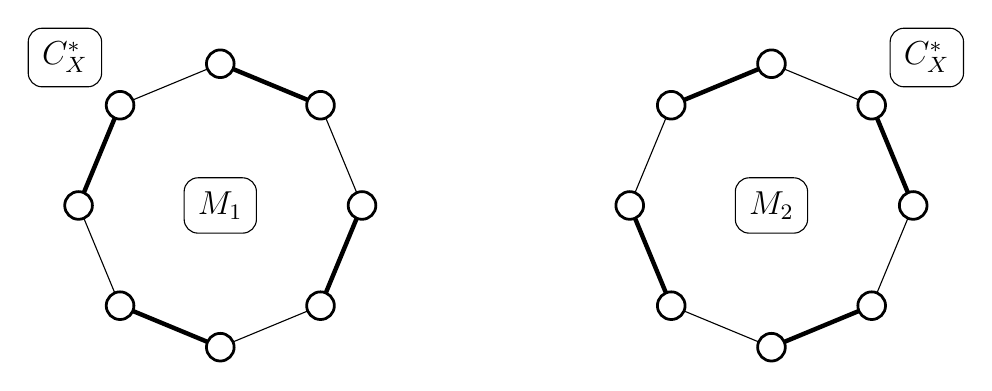
\begin{tikzpicture}[
        % 全局樣式設定
        node distance=2cm,
        % 頂點樣式:黑框白底,無填充顏色
        vertex/.style={
            circle,
            draw=black,
            fill=white,
            line width=1pt,
            minimum size=10pt,
            inner sep=0pt
        },
        % Cycle 樣式:細線 (根據你的要求)
        cycle_edge/.style={
            draw=black,
            thin
        },
        % Matching 樣式:粗線 (根據你的要求)
        matching_edge/.style={
            draw=black,
            ultra thick
        },
        % 標籤框樣式
        label_box/.style={
            draw=black,
            rounded corners=5pt,
            inner sep=5pt,
            font=\large\bfseries
        }
    ]
        % ==========================
        % 左圖:Matching M1
        % ==========================
        \begin{scope}[local bounding box=leftgraph]
            % 1. 定義節點座標 (8個點,圓形排列)
            \foreach \i in {1,...,8} {
                % 90度開始,順時針排列
                \coordinate (n\i) at ({90 - (\i-1)*45}:1.8cm);
            }
    
            % 2. 畫 Cycle (細線) - 連接一圈
            \draw[cycle_edge] (n1) -- (n2) -- (n3) -- (n4) -- (n5) -- (n6) -- (n7) -- (n8) -- cycle;
    
            % 3. 畫 Matching M1 (粗線) - 奇數邊連接 (1-2, 3-4, ...)
            \draw[matching_edge] (n1) -- (n2);
            \draw[matching_edge] (n3) -- (n4);
            \draw[matching_edge] (n5) -- (n6);
            \draw[matching_edge] (n7) -- (n8);
    
            % 4. 畫頂點 (蓋線上層)
            \foreach \i in {1,...,8} {
                \node[vertex] at (n\i) {};
            }
    
            % 5. 標籤
            \node[label_box] at (0,0) {$M_1$};
            \node[label_box, anchor=south east] at (-1.5, 1.5) {$C^*_X$};
        \end{scope}
    
    
        % ==========================
        % 右圖:Matching M2
        % ==========================
        \begin{scope}[xshift=7cm, local bounding box=rightgraph]
            % 1. 定義節點座標
            \foreach \i in {1,...,8} {
                \coordinate (m\i) at ({90 - (\i-1)*45}:1.8cm);
            }
    
            % 2. 畫 Cycle (細線)
            \draw[cycle_edge] (m1) -- (m2) -- (m3) -- (m4) -- (m5) -- (m6) -- (m7) -- (m8) -- cycle;
    
            % 3. 畫 Matching M2 (粗線) - 偶數邊連接 (2-3, 4-5, ...)
            \draw[matching_edge] (m2) -- (m3);
            \draw[matching_edge] (m4) -- (m5);
            \draw[matching_edge] (m6) -- (m7);
            \draw[matching_edge] (m8) -- (m1);
    
            % 4. 畫頂點
            \foreach \i in {1,...,8} {
                \node[vertex] at (m\i) {};
            }
    
            % 5. 標籤
            \node[label_box] at (0,0) {$M_2$};
            \node[label_box, anchor=south west] at (1.5, 1.5) {$C^*_X$};
        \end{scope}
    
    \end{tikzpicture}
    \caption{Partitioning $C^*_{X}$ into Two Perfect Matchings $M_1$ and $M_2$}
\end{figure}


Approximation 分為很多種:
\begin{itemize}
    \item Polynomial-time Approximation Scheme (PTAS):對於任意的 $\epsilon > 0$,存在一個多項式時間的演算法,可以找到一個 $(1 + \epsilon)$-approximation 的解:Euclidean TSP
    \item Constant Factor Approximation:存在一個常數 $c$,使得演算法可以找到一個 $c$-approximation 的解:Vertex Cover
    \item Logarithmic Approximation:存在一個對數函數 $\log(n)$,使得演算法可以找到一個 $\Theta(\log n)$-approximation 的解:Set Cover
    \item No Approximation Possible:除非 P = NP,否則不存在任何多項式時間的近似演算法:General TSP
\end{itemize}

\section{No Approximation Possible}

\subsection{General TSP}

\begin{exercise}[General TSP]
    Given
    \begin{itemize}
        \item \textbf{Input}: A graph $G = (V, E)$ (not necessarily complete) with non-negative edge weights. ($w$ may not satisfy the triangle inequality)
        \item \textbf{Output}: A minimum-weight Hamiltonian cycle in $G$.
    \end{itemize}
\end{exercise}

這個問題就變成 NP-Complete 問題,就算我們的近似是非常差的近似,例如 \[
    f(n) = n^n
\]
但尋找 $f(n)$-approximation algorithm 仍然是 NP-Complete 問題,因為如果有一個 $f(n)$-approximation algorithm $B$ for TSP,我們就可以拿來解 Hamiltonian Cycle on unweighted Graph 問題:
\begin{itemize}
    \item 如果 $B(G)$ 算出某個 Hamiltonian cycle $C$ 滿足 \[
        w(C) \leq f(n) \cdot w(C^*)
    \]
    就知道 $G$ 有 Hamiltonian cycle
    \item 如果 $B(G)$ 算不出任何 Hamiltonian cycle $C$ 滿足 \[
        w(C) \leq f(n) \cdot w(C^*)
    \]
    則代表 $G$ 沒有 Hamiltonian cycle,因為如果有任何 Hamiltonian cycle $C$,則 \[
        w(C) = n = w(C^*)
    \]
\end{itemize}

簡而言之,如果有 $f(n)$-approximation algorithm for General TSP,我們就可以用它來解決是否有 Hamiltonian cycle 的問題,因為有 Hamiltonian cycle 的話,approximation algorithm 一定可以找到一個比 $f(n) \cdot w(C^*)$ 還小的解(用原本就有的邊),但如果沒有 Hamiltonian cycle 的話,approximation algorithm 一定找不到比 $f(n) \cdot w(C^*)$ 還小的解(因為沒有解)。

\subsection{Logarithmic Approximation}

\begin{exercise}[Set Cover Problem]
    Given
    \begin{itemize}
        \item \textbf{Input}: $k$ subsets $S_1, S_2, \ldots, S_k$ of a Universe set $U = \{1, 2, \ldots, n\}$.
        \item \textbf{Output}: A minimum-size index set $I$ such that \[
            \bigcup_{i \in I} S_i = \{1, 2, \ldots, n\}
        \]
    \end{itemize}
\end{exercise}

\begin{theorem}
    Vertex Cover Problem $\leq_p$ Set Cover Problem.
\end{theorem}
\begin{proof}
    Given a graph $G = (V, E)$, we can construct an instance of Set Cover Problem as follows:
    \begin{itemize}
        \item Universe: $U = E$
        \item Subsets: For each vertex $v \in V$, define a subset $S_v = \{ e \in E : e \text{ is incident to } v \}$
        \item Index Set: The index set $I$ corresponds to the selected vertices in the vertex cover.
    \end{itemize}
    A vertex cover in $G$ corresponds to a set cover in the constructed instance, and vice versa. Therefore, solving the Set Cover Problem on this instance will yield a solution to the Vertex Cover Problem.
\end{proof}

所以,Set Cover Problem 是一個 NP-Hard 問題,我們可以採用以下的 Greedy Approximation Algorithm 來解決 Set Cover Problem:

\begin{algorithm}
    \DontPrintSemicolon % 隱藏每行句尾的分號 ;
    
    % 定義輸入輸出
    \KwIn{A universe set $U = \{1, 2, \ldots, n\}$ and $k$ subsets $S_1, S_2, \ldots, S_k$ of $U$}
    \KwOut{An index set $I$ such that $\bigcup_{i \in I} S_i = U$}

    $I \leftarrow \emptyset$\;
    $C \leftarrow \emptyset$\;
    \While{$C \neq U$}{
        $i \leftarrow \arg\max_{i} |S_i \setminus C|$\;
        $C \leftarrow C \cup S_i$\;
        $I \leftarrow I \cup \{i\}$\;
    }
    \Return $I$\;

    \caption{Greedy Approximation Algorithm for Set Cover Problem}
\end{algorithm}

\begin{theorem}
    The Greedy Algorithm is an $O(\log n)$-approximation algorithm for the Set Cover Problem.
\end{theorem}
\begin{proof}
    We now denote the $i$-th set chosen by the greedy algorithm as $S_{i}$, and let $C_{i}$ be the set of elements covered before the $S_i$  is chosen. Then we can let the price of choose element $j$ in the $i$-iteration is \[
        \text{price}(j) = \frac{1}{|S_i \setminus C_{i}|}
    \]
    Which will let the cost of choosing all integer be \[
        \sum_{j \in U} \text{price}(j) = |I|
    \]
    While $j$ is about to put into $C$, there are at least $n - j + 1$ elements not covered yet. $I^*$ is a collection of sets that cover all elements, so there is at least one set $t \in I^*$ that $S_t$ cover at least \[
        \frac{n - j + 1}{|I^*|}
    \]
    , which is the average number of elements that each set in $I^*$ can cover.
    
    \begin{note}
        因為 Greedy Algorithm 每次都選擇可以覆蓋最多未覆蓋元素的集合,我們已經證明一定存在起碼一個以上 cover 超過平均值的集合 $S_t$,因此 \[
            |S_i \setminus C_i| \geq |S_t \setminus C_i|
        \]
    \end{note}
    
    Therefore, we have \[
        |S_i \setminus C_i| \geq \frac{n - j + 1}{|I^*|}
    \]
    , which implies that \[
        \text{price}(j) = \frac{1}{|S_i \setminus C_i|} \leq \frac{|I^*|}{n - j + 1}
    \]
    Since the total cost is \[
        \sum_{j \in U} \text{price}(j) = |I| \leq \sum_{j=1}^{n} \frac{|I^*|}{n - j + 1} = |I^*| \cdot H_n = O(\log n) \cdot |I^*|
    \]
    , we conclude that the Greedy Algorithm is an $O(\log n)$-approximation algorithm for the Set Cover Problem.
\end{proof}

\section{Deterministic Rounding}

\begin{figure}[H]
    \centering
    \begin{tikzpicture}[
        % 全局樣式設定
        node distance=1.5cm and 2.5cm, % 垂直與水平間距
        % 1. 主要狀態方塊 (State Boxes)
        state/.style={
            rectangle,
            draw=black,
            line width=1.5pt,
            fill=white,
            minimum width=4cm,
            minimum height=1.2cm,
            align=center,
            rounded corners=3pt,
            font=\bfseries\large
        },
        % 2. 箭頭樣式 (Arrows)
        flow/.style={
            ->,
            >={Latex[length=3mm, width=2mm]}, % 使用標準 Latex 箭頭
            line width=1.2pt,
            draw=black
        },
        % 3. 動作標籤 (Action Labels - 原本的黃色氣泡)
        action/.style={
            fill=white,      % 白色背景遮擋線條
            inner sep=3pt,   % 文字與邊框距離
            font=\small\itshape, % 斜體,區分動作與名詞
            text=black
        }
    ]
    
        % --- 節點配置 (Nodes Placement) ---
        
        % 左上:ILP
        \node[state] (ilp) {Integer Linear\\Program};
        
        % 右上:LP
        \node[state, right=of ilp] (lp) {Linear\\Program};
        
        % 右下:Fractional Solution
        \node[state, below=of lp] (frac) {Fractional\\Solution};
        
        % 左下:Integral Solution
        \node[state, below=of ilp] (int) {Integral\\Solution};
    
    
        % --- 連線與標籤 (Edges & Labels) ---
        
        % 1. Relaxation: ILP -> LP
        \draw[flow] (ilp) -- node[action] {Relaxation} (lp);
        
        % 2. Solver: LP -> Fractional
        \draw[flow] (lp) -- node[action] {Solver} (frac);
        
        % 3. Rounding: Fractional -> Integral
        \draw[flow] (frac) -- node[action] {Rounding} (int);
        
        % 4. Approximation: Integral -> ILP (Closing the loop)
        \draw[flow] (int) -- node[action] {Approximation / Analysis} (ilp);
    
    \end{tikzpicture}
    \caption{The procedure of Approximation by LP Relaxation and Rounding}
\end{figure}

我們可以透過以下步驟來設計一個 approximate algorithm:
\begin{itemize}
    \item 將最佳化問題轉換成 Integer Linear Program (ILP)
    \item 將 ILP 放寬成 Linear Program (LP)
    \item 使用 polynomial-time LP solver 來求解 LP,得到 fractional solution
    \item 將 fractional solution 透過 rounding 技術轉換成 integral solution
    \item 分析 integral solution 的品質,證明其 approximation ratio
\end{itemize}

以 Vertex Cover Problem 為例,我們可以將其轉換成以下的 ILP:
\begin{exercise}[Vertex Cover ILP]
    Let \[
        x_i = \begin{cases}
            1 &\text{node } i \text{ is coverd}\\
            0 &\text{otherwise}
        \end{cases}
    \]
    The ILP formulation is as follows:
    \[
        \min \sum_{i \in V} x_i \quad \text{s.t.} \quad \begin{cases}
            x_i + x_j \geq 1 &\text{for each edge } (i, j) \in E\\
            x_i \in \{0, 1\} &\text{for each node } i \in V
        \end{cases}
    \]
\end{exercise}

然後我們可以將 ILP 放寬成一般的 LP:

\begin{exercise}[Vertex Cover LP]
    The LP formulation is as follows:
    \[
        \min \sum_{i \in V} x_i \quad \text{s.t.} \quad \begin{cases}
            x_i + x_j \geq 1 &\text{for each edge } (i, j) \in E\\
            0 \leq x_i \leq 1 &\text{for each node } i \in V
        \end{cases}
    \]
\end{exercise}

接著,我們可以使用 polynomial-time LP solver 來求解 LP,得到 fractional solution $x^* = \{x_i^*\}$

\begin{note}
    Linear Programming 可以在多項式時間內被求解,常見的演算法有 Simplex Method、Ellipsoid Method 和 Interior Point Method 這些 LP solver,但在本課程並沒有介紹,因此假設我們有一個黑盒子可以在多項式時間內求解 LP。
\end{note}

最後,我們可以透過以下的 rounding 技術來將 fractional solution 轉換成 integral solution:

Let \[
    C = \{ i \in V \mid x_i^* \geq 0.5 \}
\]


\begin{remark}
    對於每個 approximation algorithm 我們必須檢查三件事:
    \begin{itemize}
        \item \textbf{Feasibility}: $C$ 是否為一個合法的 solution
        \item \textbf{Tractability}: 運行時間是否為多項式時間
        \item \textbf{Approximation Ratio}: $|C|$ 與 $|C^*|$ 之間的關係
    \end{itemize}
\end{remark}

\newpage

\begin{theorem}
    The above rounding algorithm is a 2-approximation algorithm for the Vertex Cover Problem.
\end{theorem}
\begin{proof}
    我們證明以下三件事
    \begin{itemize}
        \item \textbf{Feasibility}: 對於每個 edge $(i, j) \in E$,根據 LP 的限制條件,我們有 \[
            x_i + x_j \geq 1
        \]
        因此至少有一個 $x_i$ 或 $x_j$ 大於等於 0.5,所以 $C$ 中至少包含一個端點,因此 $C$ 是一個合法的 vertex cover。
        \item \textbf{Tractability}: 求解 LP 的時間是多項式時間,而 rounding 的過程只需要遍歷所有的頂點,因此整體運行時間是多項式時間。
        \item \textbf{Approximation Ratio}: 由於 rouding solution $\hat{x}_i$ 有以下性質 \[
            \hat{x}_i = \begin{cases}
                1 &\text{if } x_i \geq 0.5\\
                0 &\text{otherwise}
            \end{cases}
        \]
        因此我們得到 \[
            \sum_{i \in V} \hat{x}_i \leq 2 \cdot \sum_{i \in V} x_i
        \]
        並且我們知道 \[
            \sum_{i} x_i \leq |C^*| = \sum_{i} x_i^* \leq \sum_{i} \hat{x}_i \leq 2 \cdot \sum_{i} x_i^*
        \]
        也就是 \[
            |C_{\text{LP}}| \leq |C_{\text{ILP}}| \leq |C_{\text{Rounding}}| \leq 2 \cdot |C_{\text{LP}}|
        \]
        所以我們得到 \[
            |C_{\text{Rounding}}| \leq 2 \cdot |C^*|
        \]
    \end{itemize}
    綜合以上三點,我們可以得知這是一個 2-approximation algorithm for Vertex Cover Problem。
\end{proof}

\section{Randomized Rounding}

\begin{notation}
    Suppose there are $n$ variables $1, 2, \ldots, n$. For each clause $C_j$, we denote the set as ordered pairs \((C_j^+, C_j^-)\) of disjoint subsets of variables, where \[
        C_j^+ = \{ i \mid \text{variable } i \text{ appears as a positive literal in clause } C_j \}
    \] and \[
        C_j^- = \{ i \mid \text{variable } i \text{ appears as a negative literal in clause } C_j \}
    \]
    and \[
        |C_j| = |C_j^+| + |C_j^-|
    \]
\end{notation}

\vspace{1em}

我們要解決的問題是 Max SAT Problem,因為原始的 K-SAT Problem 是 decision problem,因此我們將其轉換成 optimization problem:

\begin{exercise}[Max SAT Problem]
    Given
    \begin{itemize}
        \item \textbf{Input}: $m$ clauses $C_1, C_2, \ldots, C_m$ with $|C_j| \leq k$ over $n$ variables $1, 2, \ldots, n$.
        \item \textbf{Output}: A truth assignment that maximizes the number of satisfied clauses.
    \end{itemize}
\end{exercise}

\begin{note}
    2-SAT, MAX 1-SAT 都是 P 問題,而 3-SAT, MAX 2-SAT, MAX 3-SAT 都是 NP-Hard 問題
\end{note}

對於這個問題,有一種 0.75-approximation algorithm,精準一點來說,我們會介紹
\begin{enumerate}[label=$\arabic*^\circ$]
    \item Expected ratio $\geq 0.5$
    \item Expected ratio $\geq 1 - 1/e \approx 0.63$
    \item Expected ratio $\geq 0.75$
\end{enumerate}

\subsection{Expected Ratio $\geq 0.5$}

我們從第一種方法開始:

\begin{algorithm}
    \DontPrintSemicolon % 隱藏每行句尾的分號 ;
    
    % 定義輸入輸出
    \KwIn{$m$ clauses $C_1, C_2, \ldots, C_m$ with $|C_j| \leq k$ over $n$ variables $1, 2, \ldots, n$}
    \KwOut{A truth assignment that maximizes the number of satisfied clauses}

    \For{$i$ from $1$ to $n$}{
        Set \[
            x_i = \begin{cases}
                \text{True} &\text{with } \Pr[\text{True}]=0.5\\
                \text{False} &\text{with } \Pr[\text{False}]=0.5
            \end{cases}
        \]\;
    }
    \Return Assignment $X$\;

    \caption{Random assign}
\end{algorithm}

我們來分析這個演算法的 approximation ratio:

\begin{lemma}
    Since all variables are assigned independently, the probability of clause $C_j$ being satisfies is \[
        1 - \left( \frac{1}{2} \right)^{|C_j|}
    \]
    which is at least $\frac{1}{2}$.
\end{lemma}

所以 the expected number of satisfied clauses is at least \[
    \sum_{j=1}^{m} \left( 1 - \left( \frac{1}{2} \right)^{|C_j|} \right) \geq \sum_{j=1}^{m} \frac{1}{2} = \frac{m}{2}
\]
因此,這是一個 expected ratio $\geq 0.5$ 的 approximate algorithm for Max SAT Problem。

\newpage

\subsection{Expected Ratio $\geq 1 - 1/e$}

這個方法其實只在在 Rouning 的部分做了 Randomized Rounding:

\begin{figure}[H]
    \centering
    \begin{tikzpicture}[
        % 全局樣式設定
        node distance=1.5cm and 2.5cm, % 垂直與水平間距
        % 1. 主要狀態方塊 (State Boxes)
        state/.style={
            rectangle,
            draw=black,
            line width=1.5pt,
            fill=white,
            minimum width=4cm,
            minimum height=1.2cm,
            align=center,
            rounded corners=3pt,
            font=\bfseries\large
        },
        % 2. 箭頭樣式 (Arrows)
        flow/.style={
            ->,
            >={Latex[length=3mm, width=2mm]}, % 使用標準 Latex 箭頭
            line width=1.2pt,
            draw=black
        },
        % 3. 動作標籤 (Action Labels - 原本的黃色氣泡)
        action/.style={
            fill=white,      % 白色背景遮擋線條
            inner sep=3pt,   % 文字與邊框距離
            font=\small\itshape, % 斜體,區分動作與名詞
            text=black
        }
    ]
    
        % --- 節點配置 (Nodes Placement) ---
        
        % 左上:ILP
        \node[state] (ilp) {Integer Linear\\Program};
        
        % 右上:LP
        \node[state, right=5cm of ilp] (lp) {Linear\\Program};
        
        % 右下:Fractional Solution
        \node[state, below=of lp] (frac) {Fractional\\Solution};
        
        % 左下:Integral Solution
        \node[state, below=of ilp] (int) {Integral\\Solution};
    
    
        % --- 連線與標籤 (Edges & Labels) ---
        
        % 1. Relaxation: ILP -> LP
        \draw[flow] (ilp) -- node[action] {Relaxation} (lp);
        
        % 2. Solver: LP -> Fractional
        \draw[flow] (lp) -- node[action] {Solver} (frac);
        
        % 3. Rounding: Fractional -> Integral
        \draw[flow] (frac) -- node[action] {\textbf{\red{Randomized}} Rounding} (int);
        
        % 4. Approximation: Integral -> ILP (Closing the loop)
        \draw[flow] (int) -- node[action] {Approximation / Analysis} (ilp);
    
    \end{tikzpicture}
    \caption{The procedure of Approximation by LP Relaxation and Rounding}
\end{figure}

We first let \[
    x_i = \begin{cases}
        1 &\text{variable } i \text{ is True}\\
        0 &\text{variable } i \text{ is False}
    \end{cases}
\]
and \[
    y_j = \begin{cases}
        1 &\text{clause } C_j \text{ is satisfied}\\
        0 &\text{otherwise}
    \end{cases}
\]

\begin{exercise}[Max SAT ILP]
    The ILP formulation is as follows:
    \[
        \max \sum_{j=1}^{m} y_j \quad \text{s.t.} \quad \sum_{i \in C_j^+} x_i + \sum_{i \in C_j^-} (1 - x_i) \geq y_j
    \]
    with \[
        \begin{cases}
            x_i \in \{0, 1\} \\
            y_j \in \{0, 1\}
        \end{cases}
    \]
\end{exercise}

Then do the relaxation:

\begin{exercise}[Max SAT LP]
    The LP formulation is as follows:
    \[
        \max \sum_{j=1}^{m} y_j \quad \text{s.t.} \quad \sum_{i \in C_j^+} x_i + \sum_{i \in C_j^-} (1 - x_i) \geq y_j
    \]
    with \[
        \begin{cases}
            0 \leq x_i \leq 1 \\
            0 \leq y_j \leq 1
        \end{cases}
    \]
\end{exercise}

\begin{lemma}
    Let $(x^*, y^*)$ be the optimal solution to the LP. The maximum number of satisfied clauses (actual maximum) is at most \(\sum_{j=1}^{m} y_j^*\).
\end{lemma}
\begin{proof}
    Since the LP is a relaxation of the ILP, any feasible solution to the ILP is also a feasible solution to the LP. Therefore, the optimal value of the LP is at least as large as the optimal value of the ILP.
\end{proof}

\begin{algorithm}
    \DontPrintSemicolon % 隱藏每行句尾的分號 ;

    \For{$i$ from $1$ to $n$}{
        Set $x_i$ to be TRUE with probability $x_i^*$\;
    }
    \Return Assignment $X$\;

    \caption{Randomized Rounding}
\end{algorithm}

\begin{lemma}
    We have the inequality:
    \[
        \Pr[C_j \text{ is satisfied}] \geq \left( 1 - \left( 1 - \frac{1}{|C_j|} \right)^{|C_j|} \right) y_j^*
    \]
    , which is at least \((1 - 1/e)\ y_j^*\).
\end{lemma}
\begin{proof}
    We start from the inequality:
    \[
        \Pr[C_j \text{ is satisfied}] \geq \left( 1 - \left( 1 - \frac{1}{|C_j|} \right)^{|C_j|} \right) y_j^*
    \]
    \begin{align*}
        1 - \text{LHS} &= \left( \prod_{i \in C^+_j} (1 - x^*_i) \right) \left( \prod_{i \in C^-_j} x^*_i \right) \\[6pt]
        &\leq \left( \frac{\sum_{i \in C^+_j} (1 - x^*_i) + \sum_{i \in C^-_j} x^*_i}{|C_j|} \right)^{|C_j|} \tag{by AM-GM Inequality} \\[6pt]
        &= \left( 1 - \frac{\sum_{i \in C^+_j} (x^*_i) + \sum_{i \in C^-_j} (1 - x^*_i)}{|C_j|} \right)^{|C_j|} \leq \left( 1 - \frac{y^*_j}{|C_j|} \right)^{|C_j|} \tag{by LP constraint}
    \end{align*}
    
    \begin{claim}
        Let $f(r) = 1 - (1 - r/k)^k$. Then, for any $k \in \mathbb{Z}^+$, $f(r)$ is concave in $r \in [0, 1]$, we have \[
            f(r) \geq \left( 1 - (1 - 1/k)^k \right) r
        \]
    \end{claim}
    \vspace{-1em}
    \begin{tmpexplanation}
        One can verify that the claim holds at the endpoints $k = 1, 2$. Now, assume that $k > 2$. We have \[
            \begin{cases}
                f(0) = 0 \\
                f(1) = 1 - (1 - 1/k)^k
            \end{cases}
        \]
        and \begin{align*}
            \frac{\text{d}}{\text{d}r} f(r) &= (1 - r/k)^{k-1} \\[6pt]
            \frac{\text{d}^2}{\text{d}r^2} f(r) &= -\frac{k-1}{k} (1 - r/k)^{k-2} \leq 0
        \end{align*}
        which is concave in $r \in [0, 1]$.
    \end{tmpexplanation}
    By the claim, we have \[
        \text{LHS} \geq  1 - \left(1 - \frac{1}{|C_j|} \right)^{|C_j|} \geq \text{RHS}
    \]
\end{proof}

\subsection{Expected Ratio $\geq 0.75$}

我們可以將前兩種方法結合起來,得到更好的 approximation ratio:

\begin{algorithm}
    \DontPrintSemicolon % 隱藏每行句尾的分號 ;

    Let a boolean variable $b$ be TRUE with probability 0.5\;
    \eIf{$b=$ TRUE}{
        run the Random Assign Algorithm\;
    }{
        run the Randomized Rounding Algorithm\;
    }
    \Return Assignment $X$\;

    \caption{Combined Algorithm}
\end{algorithm}

\begin{theorem}
    The above combined algorithm is a \(\frac{3}{4}\)-approximation algorithm for the Max SAT Problem.
\end{theorem}
\begin{proof}
    By lemma 10.4.1, 10.4.3, we have \begin{align*}
        2 \cdot \Pr[C_j \text{ is satisfied}] &\geq 1 - \left( \frac{1}{2} \right)^{|C_j|} + \left( 1 - \left( 1 - \frac{1}{|C_j|} \right)^{|C_j|} \right) y_j^* \\[6pt]
        &\geq 1 - \left( \frac{1}{2} \right)^{|C_j|} + \left( 1 - \frac{1}{e} \right) y_j^* \tag{since \blue{lemma 10.4.3}} \\[6pt]
        &\geq \frac{3}{2} y_j^* \tag{since \blue{lemma 10.4.1} and \(1 - 1/e > 1/2\)} \\[6pt]
        \Rightarrow \Pr[C_j \text{ is satisfied}] &\geq \frac{3}{4} y_j^*
    \end{align*}
\end{proof}

\newpage

\section{Derandomized}

我們將使用條件期望值來進行 derandomization:

\subsection{Derandomized for Random Assign Algorithm}

\begin{figure}[H]
    \centering

    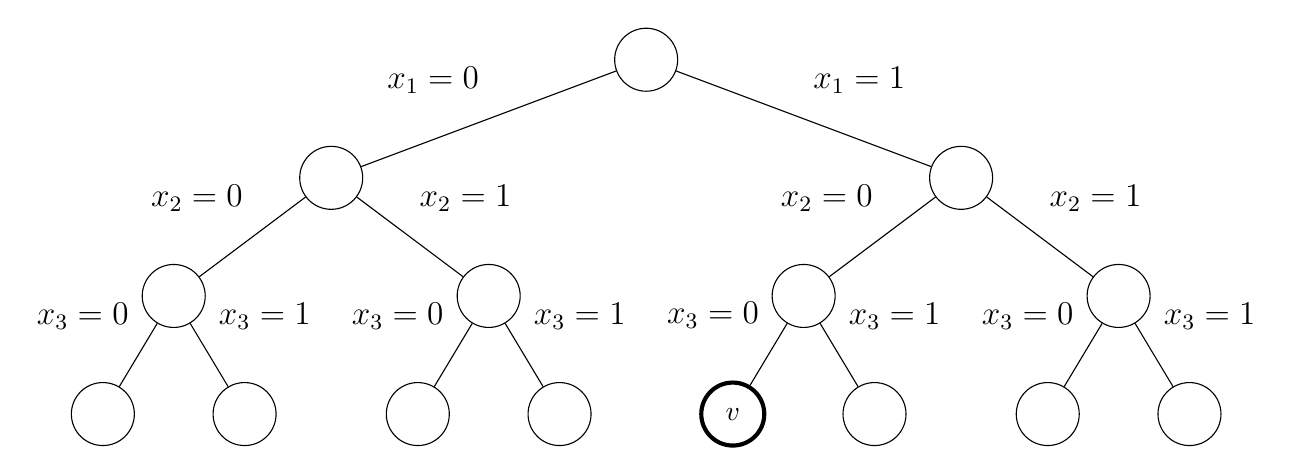
\begin{tikzpicture}[
        % 全局樣式設定
        level distance=1.5cm,    % 層與層之間的垂直距離
        % 定義每一層的水平間距,越往下越窄,避免重疊
        level 1/.style={sibling distance=8cm},
        level 2/.style={sibling distance=4cm},
        level 3/.style={sibling distance=1.8cm},
        % 節點樣式:黑框、白底、圓形
        vertex/.style={
            circle,
            draw=black,
            fill=white,       % 白色填充
            minimum size=0.8cm, % 節點大小
            inner sep=0pt
        },
        % 連線樣式
        edge from parent/.style={
            draw,
            black,
        },
        % 文字標籤樣式
        label_text/.style={
            font=\large\bfseries, % 字體大小與粗體
            midway,               % 位於線段中間
            yshift=0.2cm          % 稍微往上移一點
        }
    ]
    
        % --- 樹狀結構開始 ---
        \node[vertex] {}
            % --- 左半邊 (x1 = 0) ---
            child {
                node[vertex] {}
                child {
                    node[vertex] {}
                    % x3 層 (左左)
                    child { node[vertex] {} edge from parent node[label_text, above left] {$x_3=0$} }
                    child { node[vertex] {} edge from parent node[label_text, above right] {$x_3=1$} }
                    edge from parent node[label_text, above left] {$x_2=0$}
                }
                child {
                    node[vertex] {}
                    % x3 層 (左右)
                    child { node[vertex] {} edge from parent node[label_text, above left] {$x_3=0$} }
                    child { node[vertex] {} edge from parent node[label_text, above right] {$x_3=1$} }
                    edge from parent node[label_text, above right] {$x_2=1$}
                }
                edge from parent node[label_text, above left] {$x_1=0$}
            }
            % --- 右半邊 (x1 = 1) ---
            child {
                node[vertex] {}
                child {
                    node[vertex] {}
                    % x3 層 (右左)
                    child { node[vertex, line width=1.5pt] {$v$} edge from parent node[label_text, above left] {$x_3=0$} }
                    child { node[vertex] {} edge from parent node[label_text, above right] {$x_3=1$} }
                    edge from parent node[label_text, above left] {$x_2=0$}
                }
                child {
                    node[vertex] {}
                    % x3 層 (右右)
                    child { node[vertex] {} edge from parent node[label_text, above left] {$x_3=0$} }
                    child { node[vertex] {} edge from parent node[label_text, above right] {$x_3=1$} }
                    edge from parent node[label_text, above right] {$x_2=1$}
                }
                edge from parent node[label_text, above right] {$x_1=1$}
            };
    \end{tikzpicture}
    \caption{Truth Assignment Tree for SAT}
\end{figure}

根據上面的 Truth Assignment Tree,我們可以拿到所有可能的 truth assignment 的 decision path,而我們可以使用條件期望值來選擇每個變數的值:例如,\[
    v: x_1 = 1, x_2 = 0, x_3 = 0
\]
對每個 $v$ 來說,都可以對應一個 partial truth assignment $f(v)$

\begin{definition}[Expected Satisfied Clauses]
    For each boolean variable $x_i$, there are 0.5 probability to be TRUE or FALSE. 
    \begin{eg}
        For 
        \begin{itemize}
            \item $C_1 = \neg x_1$: satisfied T with probability 1/2
            \item $C_2 = x_2 \lor x_3$: satisfied T with probability 3/4
            \item $C_3 = x_1 \lor \neg x_2 \lor \neg x_3$: satisfied T with probability 7/8
        \end{itemize}
        because Expected number of satisfied clauses is a linear function, so we have \[
            \mathbb{E}[\text{number of satisfied clauses}] = \frac{1}{2} + \frac{3}{4} + \frac{7}{8} = \frac{13}{8}
        \]
    \end{eg}
    Expected Satisfied Clauses is the expected number of satisfied clauses.
\end{definition}

\begin{corollary}
    Since Expected Satisfied Clauses is a linear function, we have
    \begin{align*}
        \mathbb{E}[\text{number of SC}] &= \Pr[x_1 = F] \cdot \mathbb{E}[\text{number of SC} \mid x_1 = F]\\  &+ \Pr[x_1 = T] \cdot \mathbb{E}[\text{number of SC} \mid x_1 = T]    
    \end{align*}
\end{corollary}

So the conditional expectation is set to 
\begin{eg}
    If $x_1$ is set to FALSE \begin{itemize}
        \item $C_1 = \neg x_1$: satisfied T with probability 1
        \item $C_2 = x_2 \lor x_3$: satisfied T with probability 3/4
        \item $C_3 = x_1 \lor \neg x_2 \lor \neg x_3$: satisfied T with probability 3/4
    \end{itemize}
    Under this condition, we have \[
        \mathbb{E}[\text{number of SC} \mid x_1 = F] = 1 + \frac{3}{4} + \frac{3}{4} = 5/2
    \]
\end{eg}

\begin{corollary}
    If $v$ and $w$ are the children of $u$, where
    \begin{itemize}
        \item $uv$ corresponds to setting $x_i = 0$
        \item $uw$ corresponds to setting $x_i = 1$
    \end{itemize}
    then 
    \[
        \mathbb{E}[u] \leq \max \{ \mathbb{E}[v], \mathbb{E}[w] \}
    \]
\end{corollary}
\begin{proof}
    Follow the definition of conditional expectation.
    \begin{align*}
        \mathbb{E}[u] &= \Pr[x_i = 0] \cdot \mathbb{E}[v] + \Pr[x_i = 1] \cdot \mathbb{E}[w]\\[6pt]
        &= \frac{1}{2} \cdot (\mathbb{E}[v] + \mathbb{E}[w]) \\[6pt]
        &\leq \max(\mathbb{E}[v], \mathbb{E}[w])
    \end{align*}
    Proof complete.
\end{proof}

每個 node 的期望值都可以用 polynomial time 計算出來,因此找到最大期望值的路徑也可以在 polynomial time 內完成。

\begin{algorithm}
    \DontPrintSemicolon % 隱藏每行句尾的分號 ;

    Build the Truth Assignment Tree\;
    $u \leftarrow$ root of the tree\;
    \While{$u$ is not a leaf}{
        $v, w \leftarrow$ children of $u$\;
        \eIf{$\mathbb{E}[v] \geq \mathbb{E}[w]$}{
            $u \leftarrow v$\;
        }{
            $u \leftarrow w$\;
        }
    }
    \Return Assignment $f(u)$\;

    \caption{Derandomized for Random Assign Algorithm}
\end{algorithm}

\subsection{Derandomized for Randomized Rounding Algorithm}

這根第一個 derandomization 類似,我們也是建立 Truth Assignment Tree,然後使用條件期望值來選擇每個變數的值。

所以我們必須考慮的問題是,如何計算每個 node 的期望值:
\[
    \Pr[C_j \text{ is satisfied}] = 1 - \left( \prod_{i \in C^+_j} (1 - x_i^*) \right) \left( \prod_{i \in C^-_j} x_i^* \right)
\]
所以每個點的左右 probability 分別是
\begin{itemize}
    \item left child: $x_i = 0$ with probability $1 - x_i^*$
    \item right child: $x_i = 1$ with probability $x_i^*$
\end{itemize}
可以透過 linear programming 來算出來,都在 polynomial time 內。

\begin{algorithm}
    \DontPrintSemicolon % 隱藏每行句尾的分號 ;

    Build the Truth Assignment Tree\;
    $u \leftarrow$ root of the tree\;
    \While{$u$ is not a leaf}{
        $v, w \leftarrow$ children of $u$\;
        \eIf{$\mathbb{E}[v] \geq \mathbb{E}[w]$}{
            $u \leftarrow v$\;
        }{
            $u \leftarrow w$\;
        }
    }
    \Return Assignment $f(u)$\;

    \caption{Derandomized for Randomized Rounding Algorithm}
\end{algorithm}

可以發現完全一樣的演算法,只是計算每個 node 的期望值的方式不同而已。

\subsection{Derandomized for Combined Algorithm}

這次只是在最一開始的時候,選擇要跑哪一個 derandomized algorithm,我們一樣可以用條件期望值來決定:
\begin{align*}
    \mathbb{E}[\text{number of SC}] &= \Pr[b = F] \cdot \mathbb{E}[\text{number of SC} \mid b = F]\\  &+ \Pr[b = T] \cdot \mathbb{E}[\text{number of SC} \mid b = T]    
\end{align*}
因此我們可以選擇 $\mathbb{E}[\text{number of SC} \mid b = F]$ 或 $\mathbb{E}[\text{number of SC} \mid b = T]$ 較大的一個來執行,因為 root node 的 expected ratio 是 0.75,所以他的兩個 child node 至少有一個的 expected ratio 也會是 $\geq 0.75$。

\begin{algorithm}
    \DontPrintSemicolon % 隱藏每行句尾的分號 ;

    $m_1 \leftarrow \mathbb{E}[\text{number of SC} \mid b = F]$\;
    $m_2 \leftarrow \mathbb{E}[\text{number of SC} \mid b = T]$\;
    \eIf{$m_1 \geq m_2$}{
        run Derandomized for Random Assign Algorithm\;
    }{
        run Derandomized for Randomized Rounding Algorithm\;
    }
    \Return Assignment $X$\;

    \caption{Derandomized for Combined Algorithm}
\end{algorithm}